\documentclass[aspectratio=169]{beamer}

\usepackage[T5]{fontenc}
\usepackage[utf8]{inputenc}
\usepackage{lmodern}

\usetheme{Madrid}

\usepackage{graphicx}
\usepackage{multicol}
\usepackage{amsmath,amssymb}

% Outline look: blue text, numbered, no balls
\setbeamertemplate{section in toc}{%
  \leavevmode\inserttocsectionnumber.~\inserttocsection\par}
\setbeamercolor{section in toc}{fg=blue}

\hypersetup{colorlinks=true, urlcolor=blue}

\newcommand{\backbtn}{%
  \hfill\hyperlink{outline}{\beamerbutton{Mục lục}}}


% Giảm khoảng cách trên/dưới công thức hiển thị để slide gọn hơn
\makeatletter
\def\tight@disp{\setlength\abovedisplayskip{4pt plus 2pt}%
  \setlength\belowdisplayskip{4pt plus 2pt}%
  \setlength\abovedisplayshortskip{2pt plus 1pt}%
  \setlength\belowdisplayshortskip{2pt plus 1pt}}
\g@addto@macro\normalsize{\tight@disp}
\g@addto@macro\small{\tight@disp}
\g@addto@macro\footnotesize{\tight@disp}
\g@addto@macro\scriptsize{\tight@disp}
\makeatother

\title[Cột]{Cột}
\author[© N. V. Sỹ]{Nguyễn Văn Sỹ}
\institute[TNUT]{%
  Bộ môn Hệ thống Công nghiệp \\
  Trường Đại học Kỹ thuật Công nghiệp \\
  \href{mailto:vansy@tnut.edu.vn}{vansy@tnut.edu.vn}}
\date[Cơ học vật liệu]{\large Cơ học vật liệu – Ổn định của cột \\[0.5em] \footnotesize \copyright\ Nguyễn Văn Sỹ}

\begin{document}

\begin{frame}
  \titlepage
\end{frame}
%====================
\begin{frame}{Tài liệu tham khảo}
	\small
	F. P. Beer, E. R. Johnston, Jr., J. T. DeWolf, D. F. Mazurek,
	\emph{Mechanics of Materials}, 6th ed., McGraw-Hill, New York, 2012.
	
	\vspace{1em}
	\footnotesize\color{gray}
	Toàn bộ hình vẽ trong bài giảng được trích từ giáo trình trên, chỉ sử dụng
	cho mục đích giảng dạy nội bộ.
\end{frame}
% ===== OUTLINE SLIDE =====
\begin{frame}[t]{Nội dung}
  \hypertarget{outline}{}
  \scriptsize
  \begin{multicols}{2}
    \tableofcontents[hideallsubsections]
  \end{multicols}
\end{frame}

% ===== CONTENT SLIDES =====
\section{Ổn định của kết cấu}
\begin{frame}[t]{Ổn định của kết cấu}
  \begin{columns}[T]
    \column{0.58\textwidth}
      \small
      \begin{itemize}
        \setlength{\itemsep}{0.6em}
        \item Khi thiết kế cột, diện tích mặt cắt ngang được chọn sao cho:
              \begin{itemize}
                \item không vượt quá ứng suất cho phép
                \[
                  \sigma = \frac{P}{A} \le \sigma_{\mathrm{all}}
                \]
                \item biến dạng nằm trong giới hạn yêu cầu
                \[
                  \delta = \frac{PL}{AE} \le \delta_{\mathrm{spec}}
                \]
              \end{itemize}
        \item Sau các tính toán thiết kế này, có thể phát hiện ra rằng cột bị
              mất ổn định khi chịu tải và đột ngột bị cong mạnh, hay bị
              \emph{oằn} (mất ổn định).
      \end{itemize}
    \column{0.40\textwidth}
      \centering
      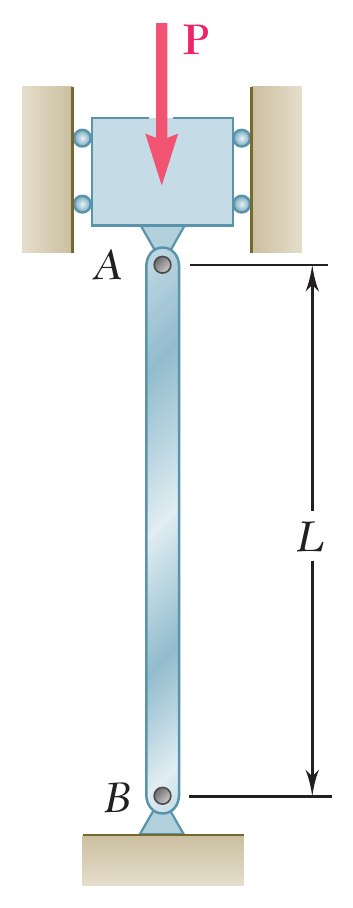
\includegraphics[width=\linewidth,height=2.9cm,keepaspectratio]{Chap_10/fig_10_1.png}\\[2pt]
      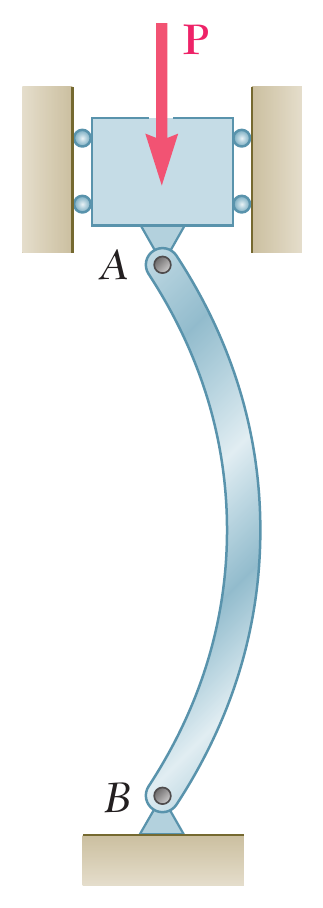
\includegraphics[width=\linewidth,height=2.9cm,keepaspectratio]{Chap_10/fig_10_2.png}
  \end{columns}
\end{frame}
% ===========
\begin{frame}[t]{Ổn định của kết cấu (tiếp)}
  \begin{columns}[T]
    \column{0.58\textwidth}
      \small
      \begin{itemize}
        \setlength{\itemsep}{0.7em}
        \item Xét mô hình gồm hai thanh và một lò xo xoắn. Sau một nhiễu động
              nhỏ:
        \[
          K(2\Delta\theta) = \text{mô men phục hồi}
        \]
        \[
          P\frac{L}{2}\sin\Delta\theta = P\frac{L}{2}\Delta\theta
            = \text{mô men gây mất ổn định}
        \]
        \item Cột ổn định (có xu hướng trở về vị trí thẳng hàng) nếu:
        \[
          P\frac{L}{2}\Delta\theta < K(2\Delta\theta)
        \]
        \[
          P < P_{cr} = \frac{4K}{L}
        \]
      \end{itemize}
    \column{0.40\textwidth}
      \centering
      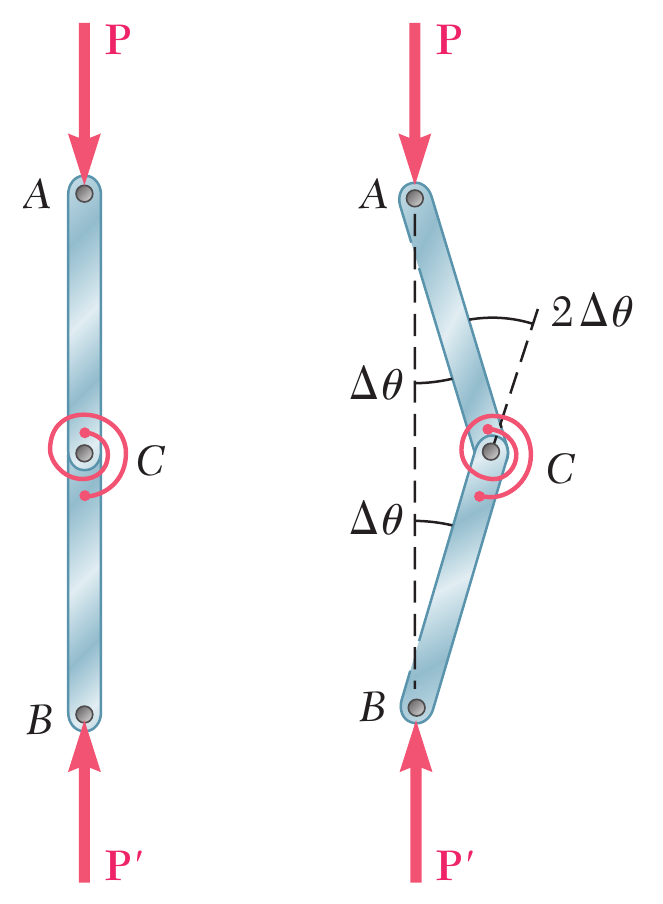
\includegraphics[width=\linewidth,height=2.9cm,keepaspectratio]{Chap_10/fig_10_4.png}\\[2pt]
      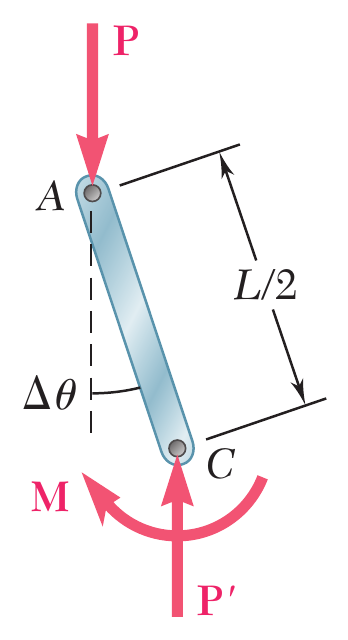
\includegraphics[width=\linewidth,height=2.9cm,keepaspectratio]{Chap_10/fig_10_5.png}
  \end{columns}
\end{frame}
% ===========
\begin{frame}[t]{Ổn định của kết cấu (tiếp)}
  \begin{columns}[T]
    \column{0.58\textwidth}
      \small
      \begin{itemize}
        \setlength{\itemsep}{0.7em}
        \item Giả sử tải trọng $P > P_{cr}$ được đặt vào. Sau một nhiễu động,
              hệ ổn định tại một cấu hình cân bằng mới với góc lệch hữu hạn:
        \[
          P\frac{L}{2}\sin\theta = K(2\theta)
        \]
        \[
          \frac{PL}{4K} = \frac{P}{P_{cr}} = \frac{\theta}{\sin\theta}
        \]
        \item Do $\sin\theta < \theta$, cấu hình giả định chỉ có thể xảy ra nếu
              $P > P_{cr}$.
      \end{itemize}
    \column{0.40\textwidth}
      \centering
      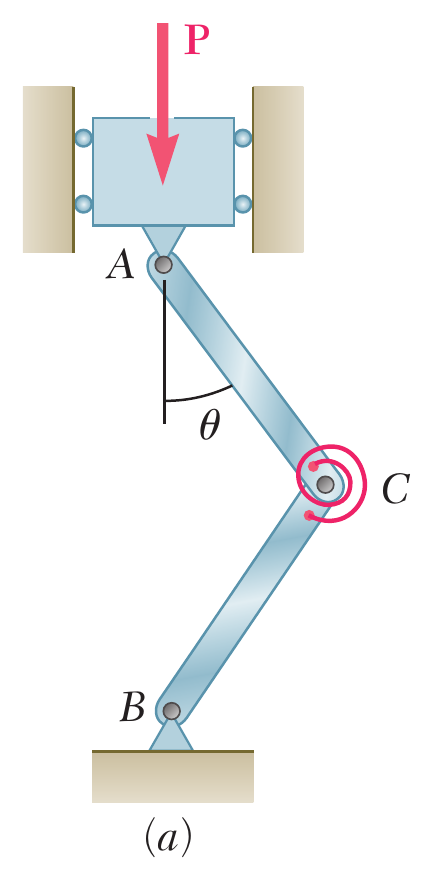
\includegraphics[width=\linewidth,height=5.5cm,keepaspectratio]{Chap_10/fig_10_6.png}
  \end{columns}
\end{frame}
% ===========
\section{Công thức Euler cho thanh hai đầu khớp}
\begin{frame}[t]{Công thức Euler cho thanh hai đầu khớp}
  \begin{columns}[T]
    \column{0.58\textwidth}
      \small
      \begin{itemize}
        \setlength{\itemsep}{0.6em}
        \item Xét một thanh chịu nén dọc trục. Sau một nhiễu động nhỏ, hệ đạt
              tới một cấu hình cân bằng sao cho:
        \[
          \frac{d^2y}{dx^2} = \frac{M}{EI} = -\frac{P}{EI}y
          \qquad
          \frac{d^2y}{dx^2} + \frac{P}{EI}y = 0
        \]
        \item Lời giải với cấu hình giả định chỉ nhận được nếu:
        \[
          P > P_{cr} = \frac{\pi^2EI}{L^2}
        \]
        \[
          \sigma = \frac{P}{A} > \sigma_{cr} = \frac{\pi^2E(Ar^2)}{L^2A}
            = \frac{\pi^2E}{(L/r)^2}
        \]
      \end{itemize}
    \column{0.40\textwidth}
      \centering
      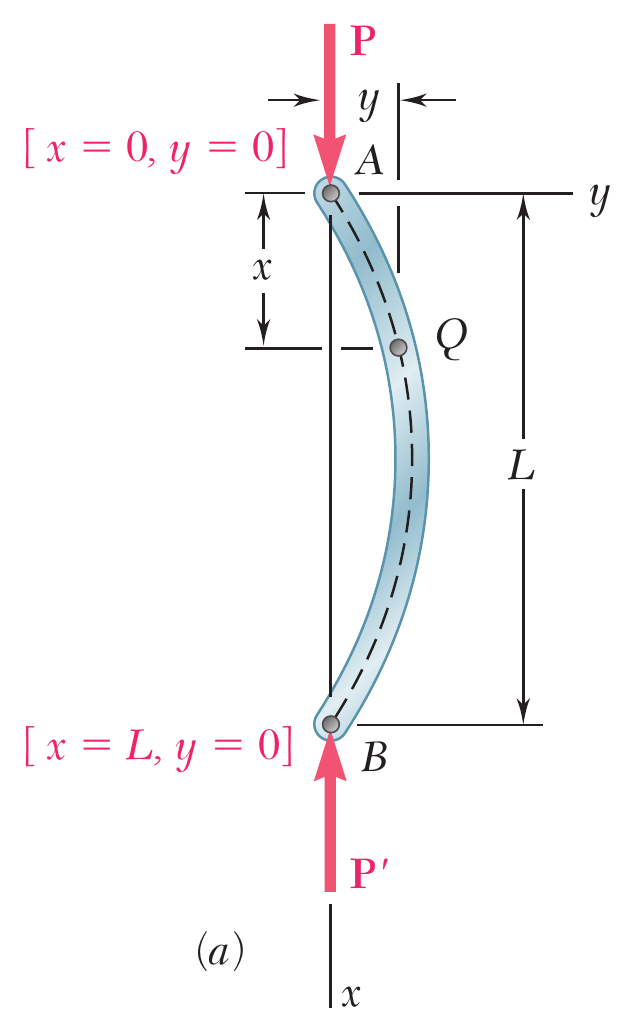
\includegraphics[width=\linewidth,height=5.5cm,keepaspectratio]{Chap_10/fig_10_7.png}
  \end{columns}
\end{frame}
% ===========
\begin{frame}[t]{Công thức Euler cho thanh hai đầu khớp (tiếp)}
  \begin{columns}[T]
    \column{0.58\textwidth}
      \small
      \begin{itemize}
        \setlength{\itemsep}{0.6em}
        \item Giá trị ứng suất ứng với tải trọng tới hạn:
        \[
          P > P_{cr} = \frac{\pi^2EI}{L^2}
        \]
        \[
          \sigma = \frac{P}{A} > \sigma_{cr} = \frac{P_{cr}}{A}
          \qquad
          \sigma_{cr} = \frac{\pi^2E}{(L/r)^2}
        \]
        $\dfrac{L}{r}$ = độ mảnh\\[0.3em]
        $\sigma_{cr}$ = ứng suất tới hạn
        \item Phân tích trên chỉ giới hạn cho tải trọng đúng tâm.
      \end{itemize}
    \column{0.40\textwidth}
      \centering
      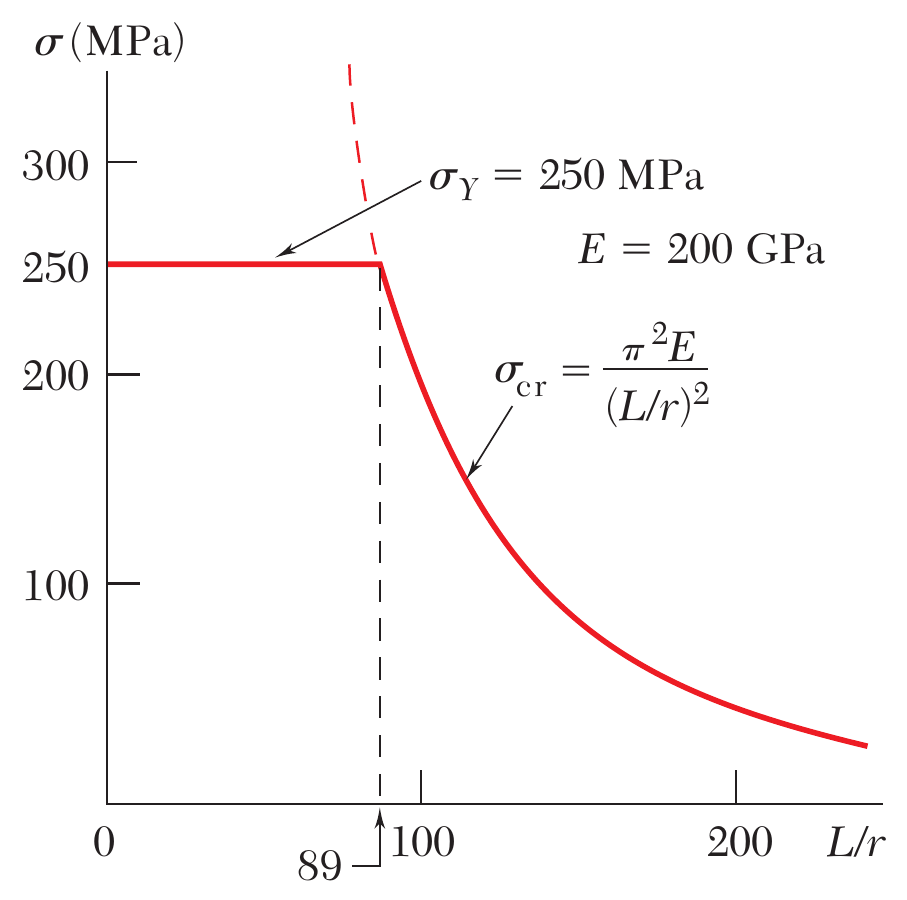
\includegraphics[width=\linewidth,height=5.5cm,keepaspectratio]{Chap_10/fig_10_8.png}
  \end{columns}
\end{frame}
% ===========
\section{Mở rộng công thức Euler}
\begin{frame}[t]{Mở rộng công thức Euler}
  \begin{columns}[T]
    \column{0.58\textwidth}
      \small
      \begin{itemize}
        \setlength{\itemsep}{0.8em}
        \item Cột có một đầu ngàm và một đầu tự do sẽ làm việc như nửa trên
              của một cột hai đầu khớp.
        \item Tải trọng tới hạn được tính theo công thức Euler:
        \[
          P_{cr} = \frac{\pi^2EI}{L_e^2}
          \qquad
          \sigma_{cr} = \frac{\pi^2E}{(L_e/r)^2}
        \]
        \[
          L_e = 2L = \text{chiều dài tương đương (chiều dài tính toán)}
        \]
      \end{itemize}
    \column{0.40\textwidth}
      \centering
      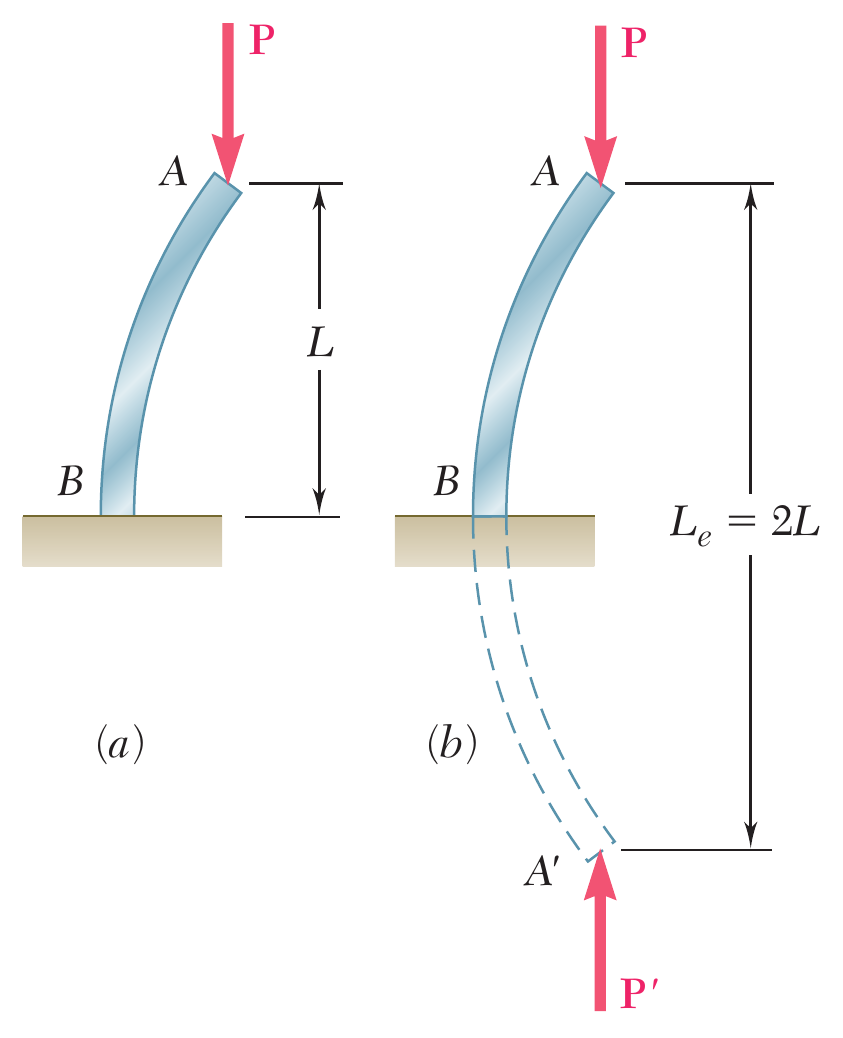
\includegraphics[width=\linewidth,height=5.5cm,keepaspectratio]{Chap_10/fig_10_9.png}
  \end{columns}
\end{frame}
% ===========
\begin{frame}[t]{Mở rộng công thức Euler (tiếp)}
  \centering
  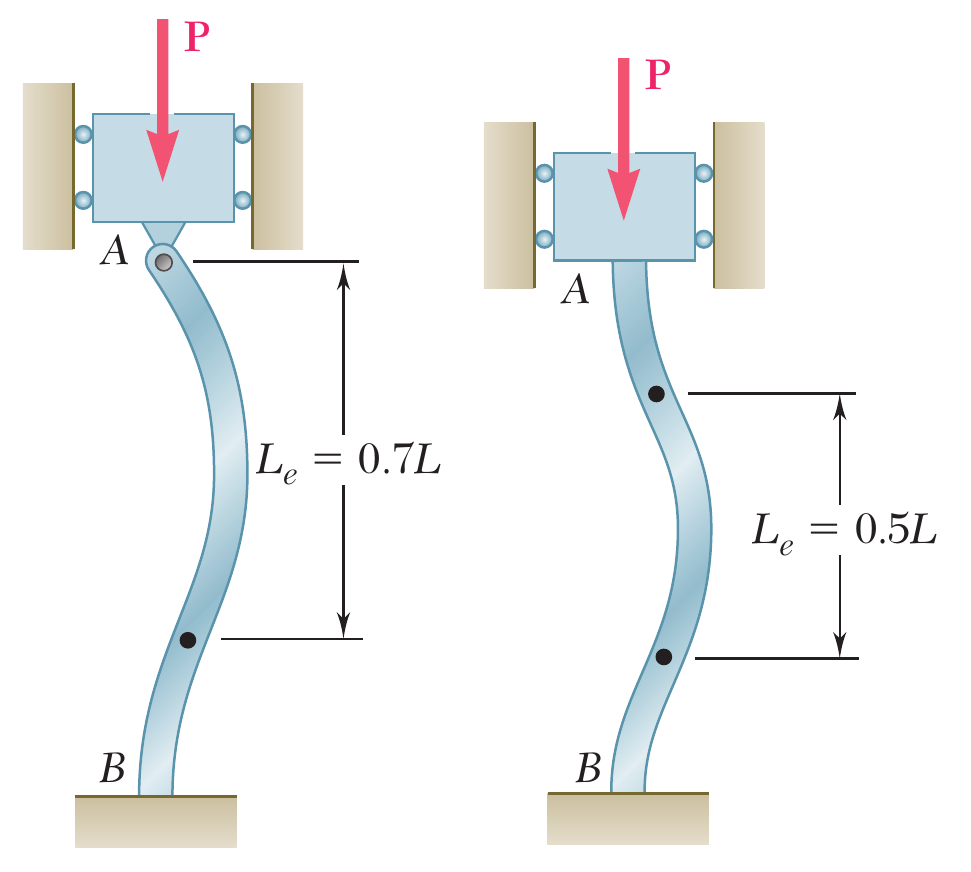
\includegraphics[width=0.9\textwidth,height=6.5cm,keepaspectratio]{Chap_10/fig_10_18.png}
\end{frame}
% ===========
\section{Bài mẫu 10.1}
\begin{frame}[t]{Bài mẫu 10.1}
  \begin{columns}[T]
    \column{0.40\textwidth}
      \centering
      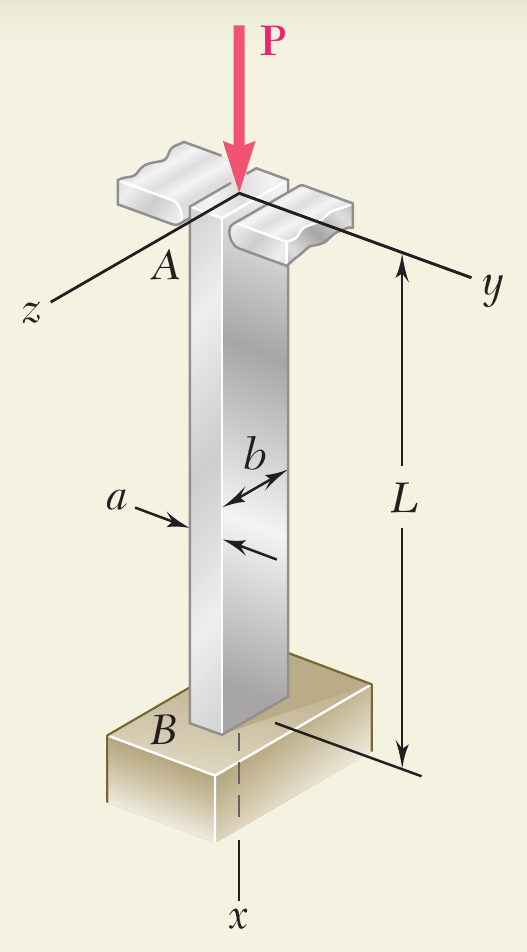
\includegraphics[width=\linewidth,height=4.6cm,keepaspectratio]{Chap_10/sp_10_1.png}\\
      \small
      $L = 0{,}5\,\mathrm{m}$, \quad $E = 70\,\mathrm{GPa}$\\
      $P = 20\,\mathrm{kN}$, \quad $FS = 2{,}5$
    \column{0.58\textwidth}
      \small
      Một cột nhôm có chiều dài $L$ và mặt cắt ngang hình chữ nhật, có đầu
      ngàm tại $B$ và chịu tải trọng đúng tâm tại $A$. Hai tấm cố định nhẵn và
      bo tròn ngăn đầu $A$ dịch chuyển trong một mặt phẳng đối xứng thẳng
      đứng nhưng cho phép nó dịch chuyển trong mặt phẳng còn lại.
      \begin{enumerate}[a)]
        \setlength{\itemsep}{0.4em}
        \item Xác định tỉ số $a/b$ của hai cạnh mặt cắt ứng với thiết kế hiệu
              quả nhất chống mất ổn định.
        \item Thiết kế mặt cắt hiệu quả nhất cho cột.
      \end{enumerate}
  \end{columns}
\end{frame}
% ===========
\begin{frame}[t]{Bài mẫu 10.1 (tiếp)}
  \begin{columns}[T]
    \column{0.60\textwidth}
      \scriptsize
      \textbf{LỜI GIẢI:}

      Thiết kế hiệu quả nhất xảy ra khi khả năng chống mất ổn định trong cả
      hai mặt phẳng đối xứng là như nhau, tức là khi các độ mảnh bằng nhau.
      \begin{itemize}
        \setlength{\itemsep}{0.15em}
        \item Mất ổn định trong mặt phẳng $xy$:
        \[
          r_z^2 = \frac{I_z}{A} = \frac{\frac{1}{12}ba^3}{ab} = \frac{a^2}{12}
          \qquad r_z = \frac{a}{\sqrt{12}}
          \qquad \frac{L_{e,z}}{r_z} = \frac{0{,}7L}{a/\sqrt{12}}
        \]
        \item Mất ổn định trong mặt phẳng $xz$:
        \[
          r_y^2 = \frac{I_y}{A} = \frac{\frac{1}{12}ab^3}{ab} = \frac{b^2}{12}
          \qquad r_y = \frac{b}{\sqrt{12}}
          \qquad \frac{L_{e,y}}{r_y} = \frac{2L}{b/\sqrt{12}}
        \]
        \item Thiết kế hiệu quả nhất:
        \[
          \frac{L_{e,z}}{r_z} = \frac{L_{e,y}}{r_y}
          \qquad
          \frac{0{,}7L}{a/\sqrt{12}} = \frac{2L}{b/\sqrt{12}}
        \]
        \[
          \frac{a}{b} = \frac{0{,}7}{2}
          \qquad \boxed{\frac{a}{b} = 0{,}35}
        \]
      \end{itemize}
    \column{0.38\textwidth}
      \centering
      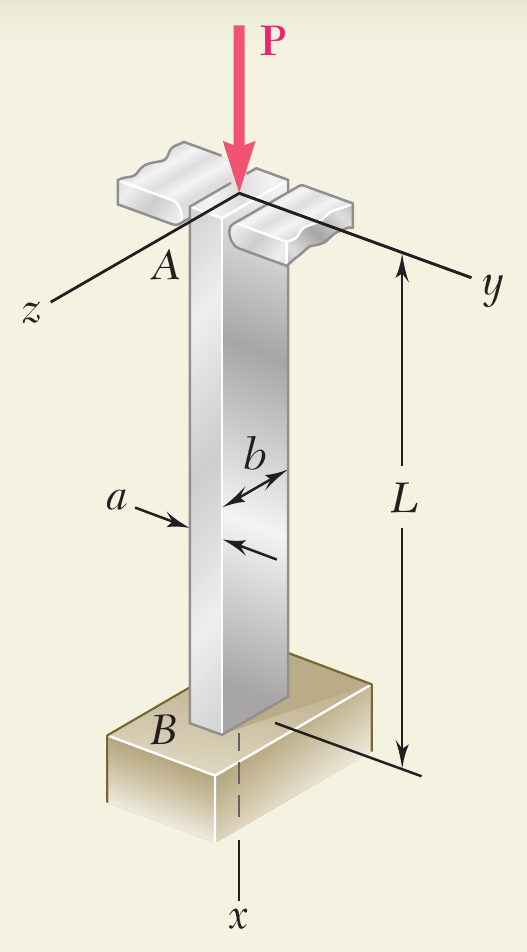
\includegraphics[width=\linewidth,height=4.7cm,keepaspectratio]{Chap_10/sp_10_1.png}
  \end{columns}
\end{frame}
% ===========
\begin{frame}[t]{Bài mẫu 10.1 (tiếp)}
  \begin{columns}[T]
    \column{0.60\textwidth}
      \small
      $L = 0{,}5\,\mathrm{m}$, $E = 70\,\mathrm{GPa}$,
      $P = 20\,\mathrm{kN}$, $FS = 2{,}5$, $a/b = 0{,}35$
      \begin{itemize}
        \setlength{\itemsep}{0.4em}
        \item Thiết kế:
        \[
          \frac{L_e}{r_y} = \frac{2L}{b/\sqrt{12}}
            = \frac{2(0{,}5\,\mathrm{m})}{b/\sqrt{12}} = \frac{3{,}464}{b}
        \]
        \[
          P_{cr} = (FS)P = (2{,}5)(20\,\mathrm{kN}) = 50\,\mathrm{kN}
        \]
        \[
          \sigma_{cr} = \frac{P_{cr}}{A} = \frac{50\,000\,\mathrm{N}}{(0{,}35b)b}
        \]
        \[
          \sigma_{cr} = \frac{\pi^2E}{(L_e/r)^2}
            = \frac{\pi^2(70\times10^{9}\,\mathrm{Pa})}{(3{,}464/b)^2}
        \]
        \[
          \frac{50\,000\,\mathrm{N}}{(0{,}35b)b}
            = \frac{\pi^2(70\times10^{9}\,\mathrm{Pa})}{(3{,}464/b)^2}
        \]
        \[
          \boxed{b = 39{,}7\,\mathrm{mm} \qquad a = 0{,}35b = 13{,}9\,\mathrm{mm}}
        \]
      \end{itemize}
    \column{0.38\textwidth}
      \centering
      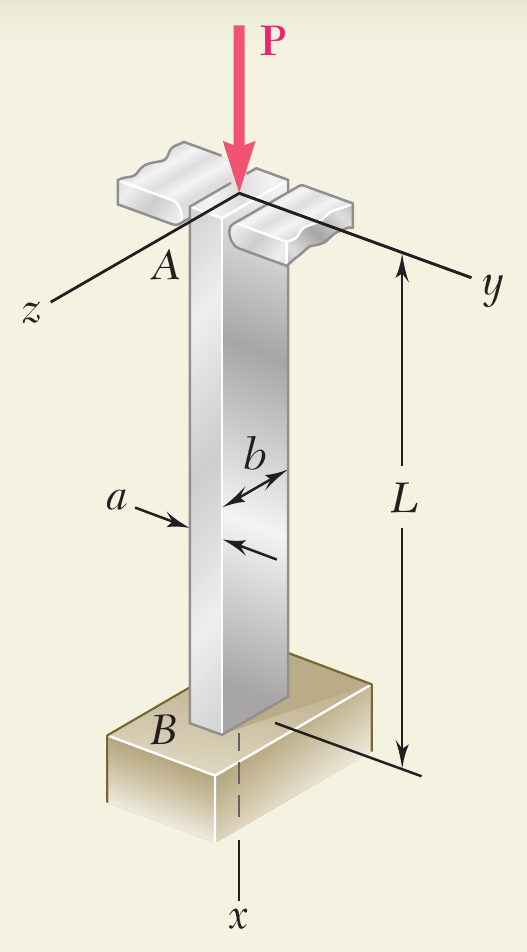
\includegraphics[width=\linewidth,height=5.5cm,keepaspectratio]{Chap_10/sp_10_1.png}
  \end{columns}
\end{frame}
% ===========
\section{Tải trọng lệch tâm: công thức secant}
\begin{frame}[t]{Tải trọng lệch tâm: công thức secant}
  \begin{columns}[T]
    \column{0.60\textwidth}
      \footnotesize
      \begin{itemize}
        \setlength{\itemsep}{0.20em}
        \item Tải trọng lệch tâm tương đương với một lực đúng tâm và một ngẫu
              lực.
        \item Uốn xảy ra với mọi độ lệch tâm khác không. Vấn đề mất ổn định trở
              thành liệu độ võng gây ra có quá lớn hay không.
        \item Độ võng trở nên vô hạn khi $P = P_{cr}$:
        \[
          y_{\max} = e\left[\sec\left(\frac{\pi}{2}\sqrt{\frac{P}{P_{cr}}}\right) - 1\right]
          \qquad
          P_{cr} = \frac{\pi^2EI}{L_e^2}
        \]
        \item Ứng suất lớn nhất:
        \[
          \sigma_{\max} = \frac{P}{A}\left[1 + \frac{(y_{\max} + e)c}{r^2}\right]
        \]
        \[
          \sigma_{\max} = \frac{P}{A}\left[1 + \frac{ec}{r^2}
            \sec\left(\frac{1}{2}\sqrt{\frac{P}{EA}}\frac{L_e}{r}\right)\right]
        \]
      \end{itemize}
    \column{0.38\textwidth}
      \centering
      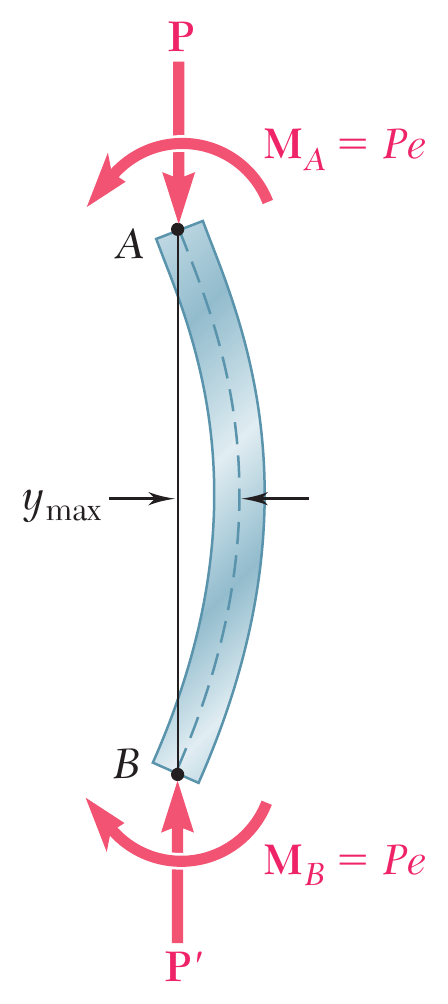
\includegraphics[width=\linewidth,height=4.7cm,keepaspectratio]{Chap_10/fig_10_19.png}
  \end{columns}
\end{frame}
% ===========
\begin{frame}[t]{Tải trọng lệch tâm: công thức secant (tiếp)}
  \begin{columns}[T]
    \column{0.40\textwidth}
      \small
      \[
        \sigma_{\max} = \sigma_Y
      \]
      \[
        = \frac{P}{A}\left[1 + \frac{ec}{r^2}
            \sec\left(\frac{1}{2}\sqrt{\frac{P}{EA}}\frac{L_e}{r}\right)\right]
      \]
    \column{0.58\textwidth}
      \centering
      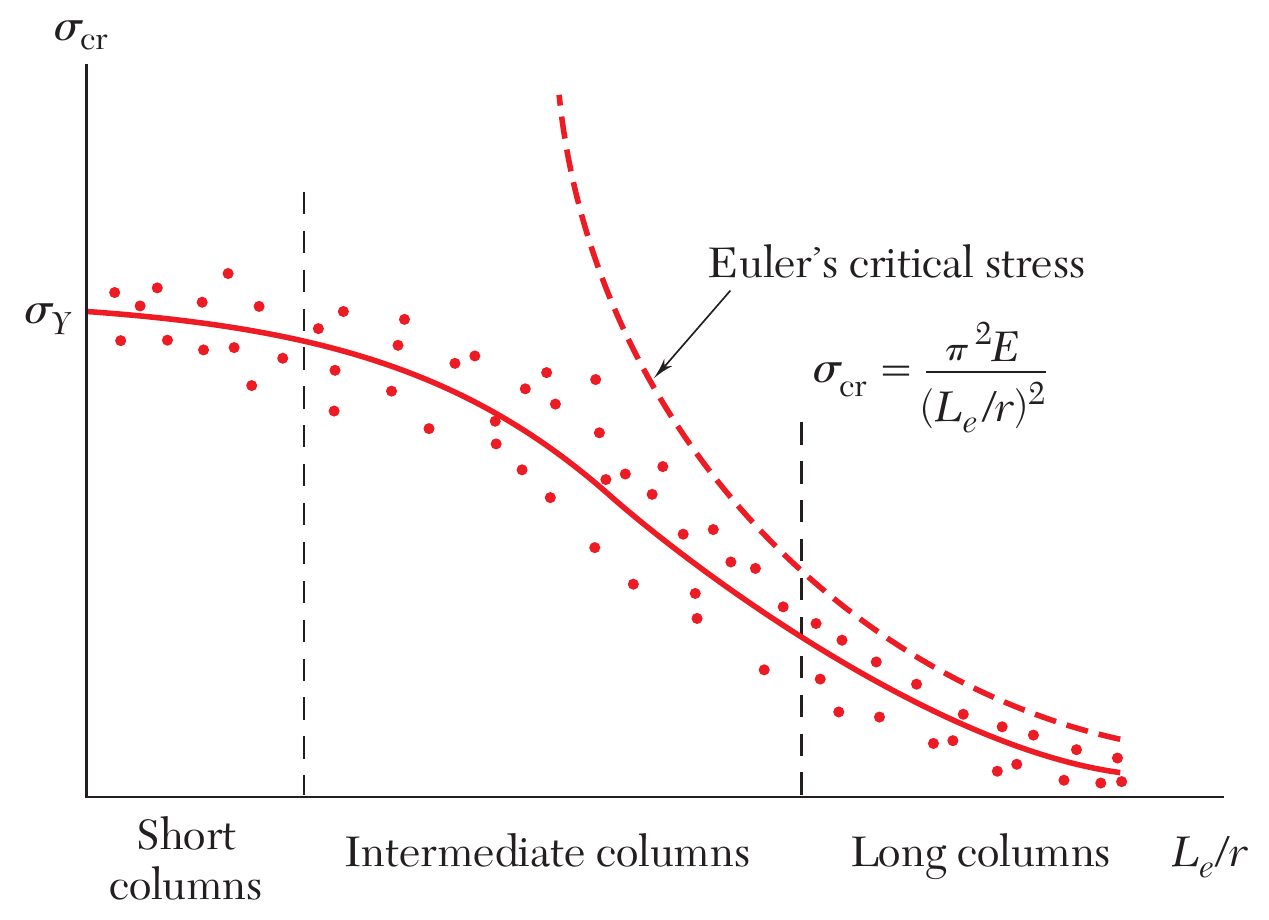
\includegraphics[width=\linewidth,height=5.8cm,keepaspectratio]{Chap_10/fig_10_24.png}\\
      \scriptsize Hình 10.24: Tải trọng trên một đơn vị diện tích, $P/A$, gây
      chảy dẻo trong cột.
  \end{columns}
\end{frame}
% ===========
\section{Bài mẫu 10.2}
\begin{frame}[t]{Bài mẫu 10.2}
  \begin{columns}[T]
    \column{0.40\textwidth}
      \centering
      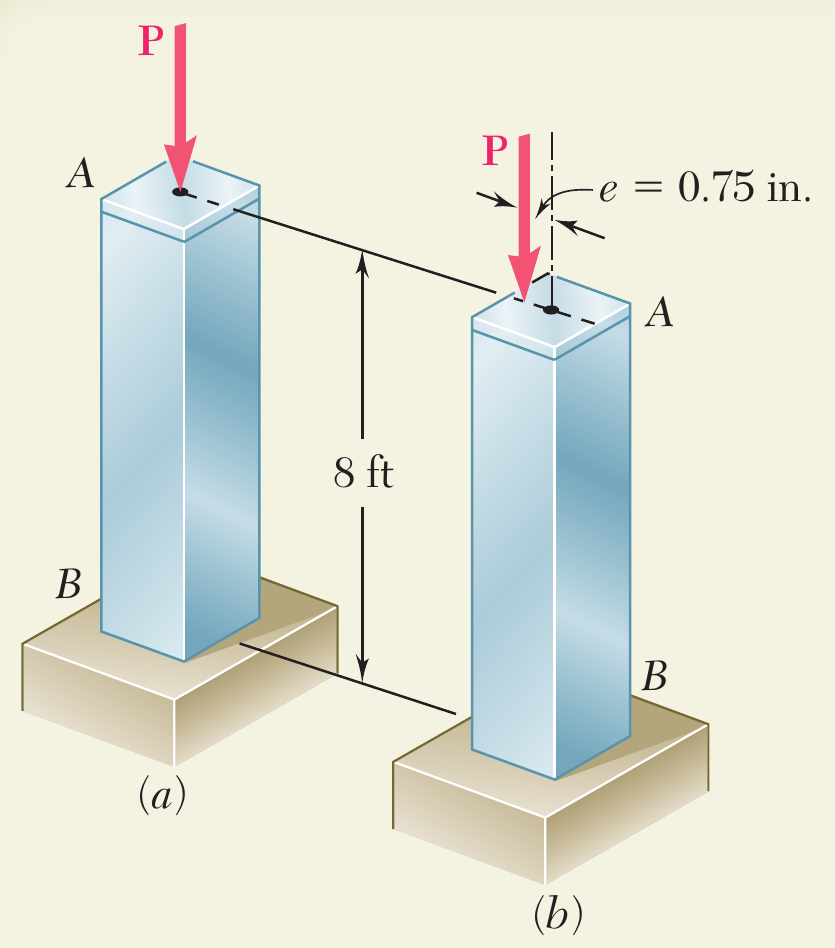
\includegraphics[width=\linewidth,height=5cm,keepaspectratio]{Chap_10/sp_10_2_a.png}\\
      \small $E = 200\,\mathrm{GPa}$
    \column{0.58\textwidth}
      \small
      Cột đồng chất gồm một đoạn ống thép kết cấu dài 2,4 m có mặt cắt ngang
      như hình vẽ.
      \begin{enumerate}[a)]
        \setlength{\itemsep}{0.5em}
        \item Sử dụng công thức Euler và hệ số an toàn bằng hai, xác định tải
              trọng đúng tâm cho phép của cột và ứng suất pháp tương ứng.
        \item Giả sử tải trọng cho phép tìm được ở câu a được đặt tại điểm cách
              trục hình học của cột 18 mm, xác định chuyển vị ngang của đỉnh cột
              và ứng suất pháp lớn nhất trong cột.
      \end{enumerate}
  \end{columns}
\end{frame}
% ===========
\begin{frame}[t]{Bài mẫu 10.2 (tiếp)}
  \begin{columns}[T]
    \column{0.58\textwidth}
      \small
      \textbf{LỜI GIẢI:}
      \begin{itemize}
        \setlength{\itemsep}{0.4em}
        \item Tải trọng đúng tâm cho phép lớn nhất:

              Chiều dài tính toán:
        \[
          L_e = 2(2{,}4\,\mathrm{m}) = 4{,}8\,\mathrm{m}
        \]
              Tải trọng tới hạn:
        \[
          P_{cr} = \frac{\pi^2EI}{L_e^2}
            = \frac{\pi^2(200\times10^{9})(3{,}33\times10^{-6})}{(4{,}8)^2}
            = 285{,}3\,\mathrm{kN}
        \]
              Tải trọng cho phép:
        \[
          P_{\mathrm{all}} = \frac{P_{cr}}{FS} = \frac{285{,}3\,\mathrm{kN}}{2}
          \qquad \boxed{P_{\mathrm{all}} = 142{,}7\,\mathrm{kN}}
        \]
        \[
          \sigma = \frac{P_{\mathrm{all}}}{A} = \frac{142\,700\,\mathrm{N}}{2284\times10^{-6}\,\mathrm{m}^2}
          \qquad \boxed{\sigma = 62{,}5\,\mathrm{MPa}}
        \]
      \end{itemize}
    \column{0.40\textwidth}
      \centering
      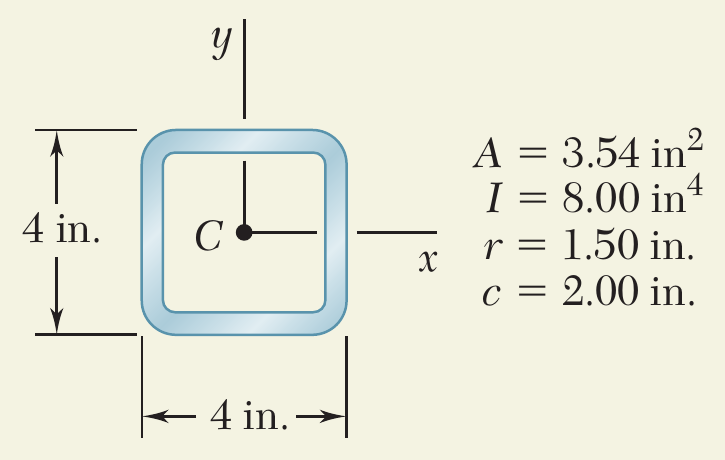
\includegraphics[width=\linewidth,height=5.5cm,keepaspectratio]{Chap_10/sp_10_2_b.png}
  \end{columns}
\end{frame}
% ===========
\begin{frame}[t]{Bài mẫu 10.2 (tiếp)}
  \begin{columns}[T]
    \column{0.60\textwidth}
      \footnotesize
      \begin{itemize}
        \setlength{\itemsep}{0.20em}
        \item Tải trọng lệch tâm:

              Chuyển vị đầu cột:
        \[
          y_m = e\left[\sec\left(\frac{\pi}{2}\sqrt{\frac{P}{P_{cr}}}\right) - 1\right]
        \]
        \[
          y_m = (0{,}018\,\mathrm{m})\left[\sec\left(\frac{\pi}{2\sqrt{2}}\right) - 1\right]
        \]
        \[
          \boxed{y_m = 22{,}5\,\mathrm{mm}}
        \]
              Ứng suất pháp lớn nhất:
        \[
          \sigma_m = \frac{P}{A}\left[1 + \frac{ec}{r^2}
            \sec\left(\frac{\pi}{2}\sqrt{\frac{P}{P_{cr}}}\right)\right]
        \]
        \[
          = \frac{142\,700\,\mathrm{N}}{2284\times10^{-6}\,\mathrm{m}^2}
            \left[1 + \frac{(0{,}018\,\mathrm{m})(0{,}05\,\mathrm{m})}{(0{,}038\,\mathrm{m})^2}
            \sec\left(\frac{\pi}{2\sqrt{2}}\right)\right]
        \]
        \[
          \boxed{\sigma_m = 150{,}2\,\mathrm{MPa}}
        \]
      \end{itemize}
    \column{0.38\textwidth}
      \centering
      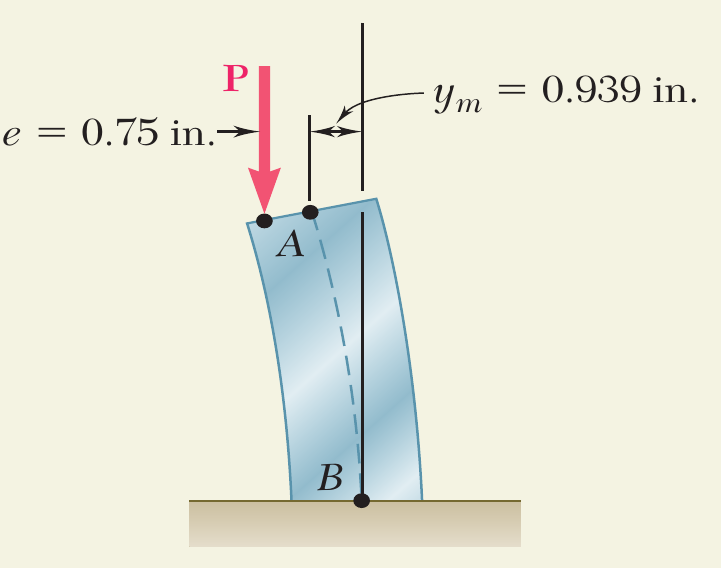
\includegraphics[width=\linewidth,height=4.7cm,keepaspectratio]{Chap_10/sp_10_2_c.png}
  \end{columns}
\end{frame}
% ===========
\section{Thiết kế cột chịu tải trọng đúng tâm}
\begin{frame}[t]{Thiết kế cột chịu tải trọng đúng tâm}
  \begin{columns}[T]
    \column{0.56\textwidth}
      \small
      \begin{itemize}
        \setlength{\itemsep}{0.6em}
        \item Các phân tích trước đây giả thiết ứng suất nhỏ hơn giới hạn tỉ
              lệ, cột ban đầu thẳng và đồng chất.
        \item Dữ liệu thực nghiệm cho thấy:
              \begin{itemize}
                \setlength{\itemsep}{0.3em}
                \item với $L_e/r$ lớn, $\sigma_{cr}$ tuân theo công thức Euler,
                      phụ thuộc vào $E$ nhưng không phụ thuộc $\sigma_Y$.
                \item với $L_e/r$ nhỏ, $\sigma_{cr}$ được quyết định bởi giới hạn
                      chảy $\sigma_Y$ chứ không phải $E$.
                \item với $L_e/r$ trung bình, $\sigma_{cr}$ phụ thuộc cả
                      $\sigma_Y$ và $E$.
              \end{itemize}
      \end{itemize}
    \column{0.42\textwidth}
      \centering
      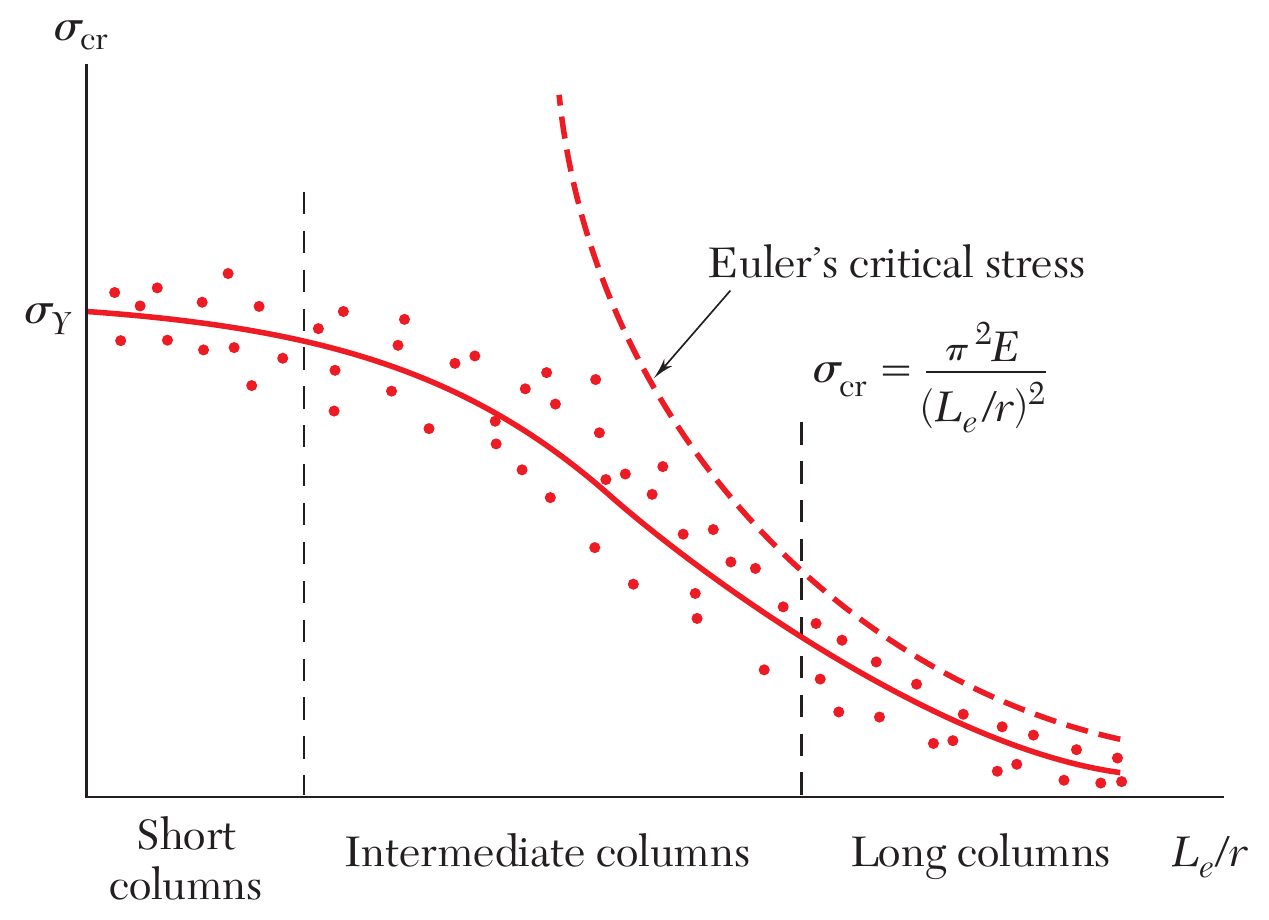
\includegraphics[width=\linewidth,height=5.5cm,keepaspectratio]{Chap_10/fig_10_24.png}
  \end{columns}
\end{frame}
% ===========
\begin{frame}[t]{Thiết kế cột chịu tải trọng đúng tâm: thép kết cấu}
  \begin{columns}[T]
    \column{0.60\textwidth}
      \footnotesize
      \textbf{Thép kết cấu} -- Viện Kết cấu Thép Hoa Kỳ (AISC)
      \begin{itemize}
        \setlength{\itemsep}{0.3em}
        \item Với $L/r > C_c$:
        \[
          \sigma_{cr} = \frac{\pi^2E}{(L/r)^2} \qquad
          \sigma_{\mathrm{all}} = \frac{\sigma_{cr}}{FS} \qquad FS = 1{,}92
        \]
        \item Với $L/r < C_c$:
        \[
          \sigma_{cr} = \sigma_Y\left[1 - \frac{(L/r)^2}{2C_c^2}\right]
          \qquad
          \sigma_{\mathrm{all}} = \frac{\sigma_{cr}}{FS}
        \]
        \[
          FS = \frac{5}{3} + \frac{3}{8}\frac{L/r}{C_c}
            - \frac{1}{8}\left(\frac{L/r}{C_c}\right)^3
        \]
        \item Tại $L/r = C_c$:
        \[
          \sigma_{cr} = \tfrac{1}{2}\sigma_Y \qquad
          C_c^2 = \frac{2\pi^2E}{\sigma_Y}
        \]
      \end{itemize}
    \column{0.38\textwidth}
      \centering
      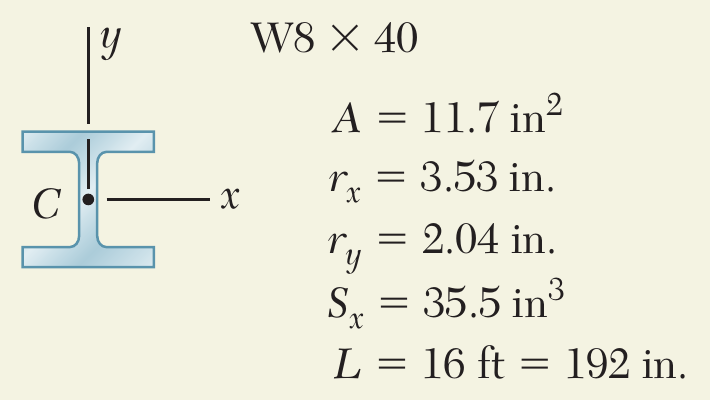
\includegraphics[width=\linewidth,height=5.5cm,keepaspectratio]{Chap_10/sp_10_7.png}
  \end{columns}
\end{frame}
% ===========
\begin{frame}[t]{Thiết kế cột chịu tải trọng đúng tâm: nhôm}
  \begin{columns}[T]
    \column{0.58\textwidth}
      \small
      \textbf{Nhôm} -- Hiệp hội Nhôm Hoa Kỳ (Aluminum Association, Inc.)
      \begin{itemize}
        \setlength{\itemsep}{0.5em}
        \item Hợp kim 6061-T6:
        \[
          L/r < 66:\quad \sigma_{\mathrm{all}} = [139 - 0{,}868(L/r)]\,\mathrm{MPa}
        \]
        \[
          L/r \ge 66:\quad \sigma_{\mathrm{all}} = \frac{351\times10^{3}\,\mathrm{MPa}}{(L/r)^2}
        \]
        \item Hợp kim 2014-T6:
        \[
          L/r < 55:\quad \sigma_{\mathrm{all}} = [212 - 1{,}585(L/r)]\,\mathrm{MPa}
        \]
        \[
          L/r \ge 55:\quad \sigma_{\mathrm{all}} = \frac{372\times10^{3}\,\mathrm{MPa}}{(L/r)^2}
        \]
      \end{itemize}
    \column{0.40\textwidth}
      \centering
      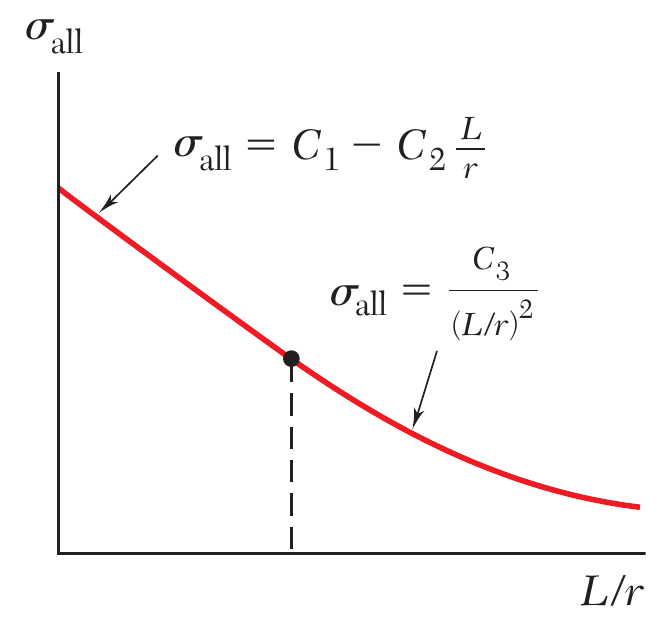
\includegraphics[width=\linewidth,height=5.5cm,keepaspectratio]{Chap_10/fig_10_29.png}
  \end{columns}
\end{frame}
% ===========
\section{Bài mẫu 10.4}
\begin{frame}[t]{Bài mẫu 10.4}
  \begin{columns}[T]
    \column{0.40\textwidth}
      \centering
      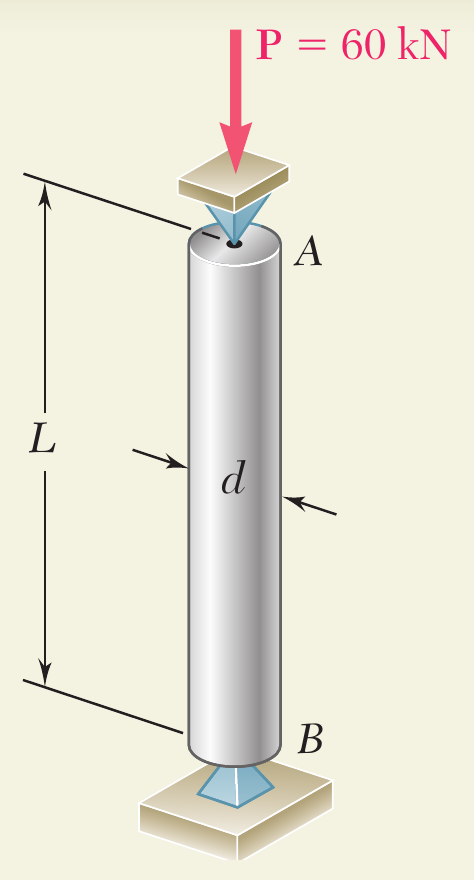
\includegraphics[width=\linewidth,height=5.5cm,keepaspectratio]{Chap_10/sp_10_4.png}
    \column{0.58\textwidth}
      \small
      Sử dụng hợp kim nhôm 2014-T6, xác định đường kính nhỏ nhất của thanh có
      thể chịu tải trọng đúng tâm $P = 60\,\mathrm{kN}$ nếu
      a) $L = 750\,\mathrm{mm}$, b) $L = 300\,\mathrm{mm}$.

      \vspace{0.8em}
      \textbf{LỜI GIẢI:}
      \begin{itemize}
        \setlength{\itemsep}{0.4em}
        \item Khi chưa biết đường kính, không thể tính độ mảnh. Phải đưa ra
              giả thiết về miền độ mảnh sẽ sử dụng.
        \item Tính đường kính cần thiết với miền độ mảnh đã giả thiết.
        \item Tính độ mảnh và kiểm tra giả thiết ban đầu. Lặp lại nếu cần.
      \end{itemize}
  \end{columns}
\end{frame}
% ===========
\begin{frame}[t]{Bài mẫu 10.4 (tiếp)}
  \begin{columns}[T]
    \column{0.60\textwidth}
      \footnotesize
      $c$ = bán kính thanh, \quad $r$ = bán kính quán tính
      \[
        r = \sqrt{\frac{I}{A}} = \sqrt{\frac{\pi c^4/4}{\pi c^2}} = \frac{c}{2}
      \]
      \begin{itemize}
        \setlength{\itemsep}{0.20em}
        \item Với $L = 750\,\mathrm{mm}$, giả thiết $L/r > 55$.
        \item Xác định bán kính thanh:
        \[
          \sigma_{\mathrm{all}} = \frac{P}{A} = \frac{372\times10^{3}\,\mathrm{MPa}}{(L/r)^2}
          \qquad
          \frac{60\times10^{3}\,\mathrm{N}}{\pi c^2}
            = \frac{372\times10^{9}\,\mathrm{Pa}}{\left(\frac{0{,}750\,\mathrm{m}}{c/2}\right)^2}
        \]
        \[
          c = 18{,}44\,\mathrm{mm}
        \]
        \item Kiểm tra giả thiết về độ mảnh:
        \[
          \frac{L}{r} = \frac{L}{c/2} = \frac{750\,\mathrm{mm}}{(18{,}44\,\mathrm{mm})/2}
            = 81{,}3 > 55
        \]
        giả thiết đúng \qquad $\boxed{d = 2c = 36{,}9\,\mathrm{mm}}$
      \end{itemize}
    \column{0.38\textwidth}
      \centering
      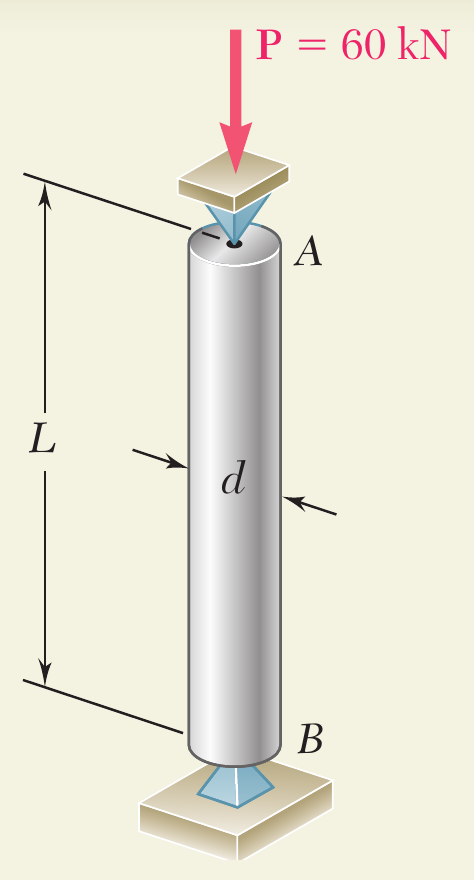
\includegraphics[width=\linewidth,height=4.7cm,keepaspectratio]{Chap_10/sp_10_4.png}
  \end{columns}
\end{frame}
% ===========
\begin{frame}[t]{Bài mẫu 10.4 (tiếp)}
  \begin{columns}[T]
    \column{0.60\textwidth}
      \small
      \begin{itemize}
        \setlength{\itemsep}{0.4em}
        \item Với $L = 300\,\mathrm{mm}$, giả thiết $L/r < 55$.
        \item Xác định bán kính thanh:
        \[
          \sigma_{\mathrm{all}} = \frac{P}{A}
            = \left[212 - 1{,}585\left(\frac{L}{r}\right)\right]\mathrm{MPa}
        \]
        \[
          \frac{60\times10^{3}\,\mathrm{N}}{\pi c^2}
            = \left[212 - 1{,}585\left(\frac{0{,}3\,\mathrm{m}}{c/2}\right)\right]\times10^{6}\,\mathrm{Pa}
        \]
        \[
          c = 12{,}00\,\mathrm{mm}
        \]
        \item Kiểm tra giả thiết về độ mảnh:
        \[
          \frac{L}{r} = \frac{L}{c/2} = \frac{300\,\mathrm{mm}}{(12{,}00\,\mathrm{mm})/2}
            = 50 < 55
        \]
        giả thiết đúng \qquad $\boxed{d = 2c = 24{,}0\,\mathrm{mm}}$
      \end{itemize}
    \column{0.38\textwidth}
      \centering
      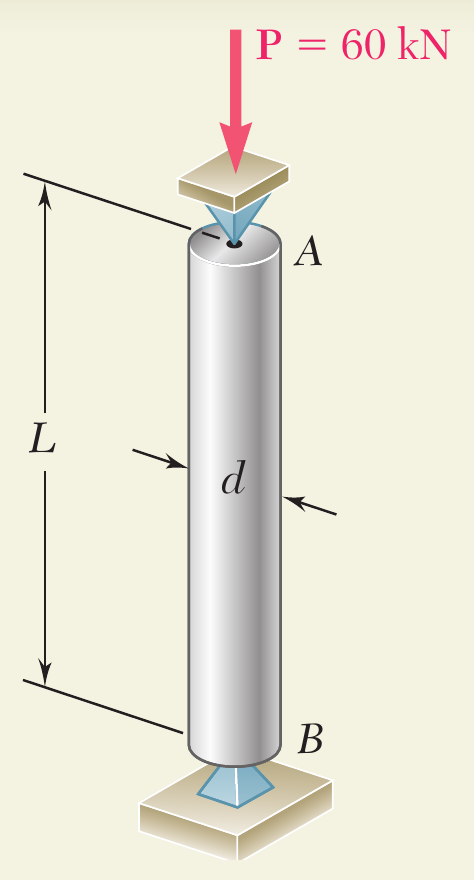
\includegraphics[width=\linewidth,height=5.5cm,keepaspectratio]{Chap_10/sp_10_4.png}
  \end{columns}
\end{frame}
% ===========
\section{Thiết kế cột chịu tải trọng lệch tâm}
\begin{frame}[t]{Thiết kế cột chịu tải trọng lệch tâm}
  \begin{columns}[T]
    \column{0.58\textwidth}
      \small
      \begin{itemize}
        \setlength{\itemsep}{0.5em}
        \item Tải trọng lệch tâm $P$ có thể được thay bằng một lực đúng tâm $P$
              và một ngẫu lực $M = Pe$.
        \item Ứng suất pháp có thể tìm bằng cách cộng tác dụng ứng suất do lực
              đúng tâm và do ngẫu lực:
        \[
          \sigma = \sigma_{\text{đúng tâm}} + \sigma_{\text{uốn}}
          \qquad
          \sigma_{\max} = \frac{P}{A} + \frac{Mc}{I}
        \]
        \item Phương pháp ứng suất cho phép:
        \[
          \frac{P}{A} + \frac{Mc}{I} \le \sigma_{\mathrm{all}}
        \]
        \item Phương pháp tương tác:
        \[
          \frac{P/A}{(\sigma_{\mathrm{all}})_{\text{đúng tâm}}}
            + \frac{Mc/I}{(\sigma_{\mathrm{all}})_{\text{uốn}}} \le 1
        \]
      \end{itemize}
    \column{0.40\textwidth}
      \centering
      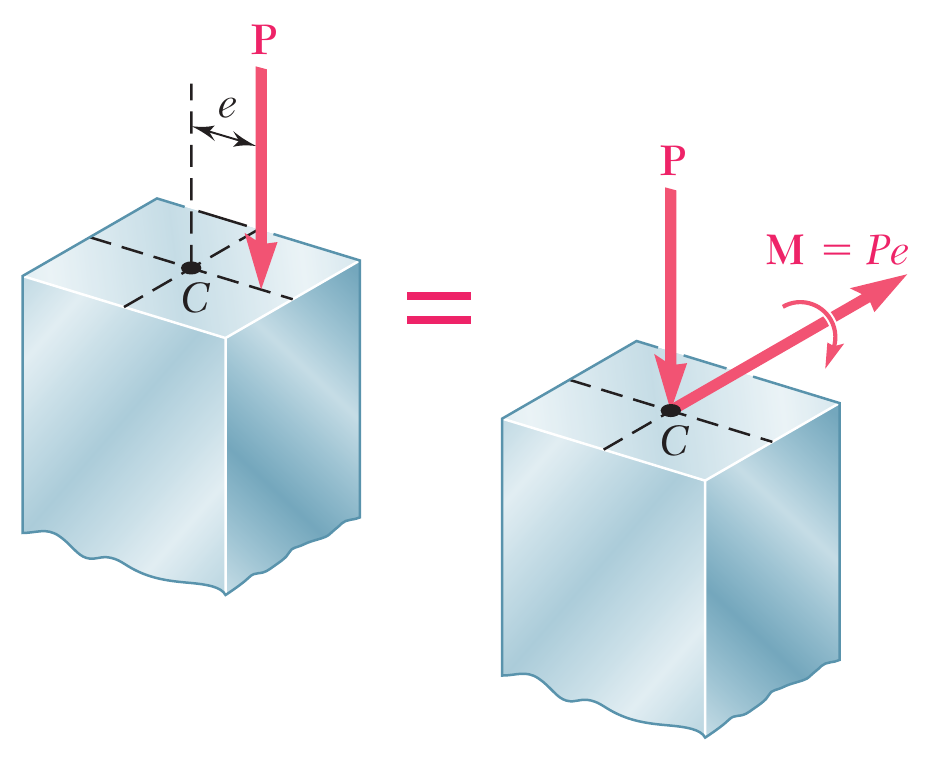
\includegraphics[width=\linewidth,height=2.9cm,keepaspectratio]{Chap_10/fig_10_32.png}\\[2pt]
      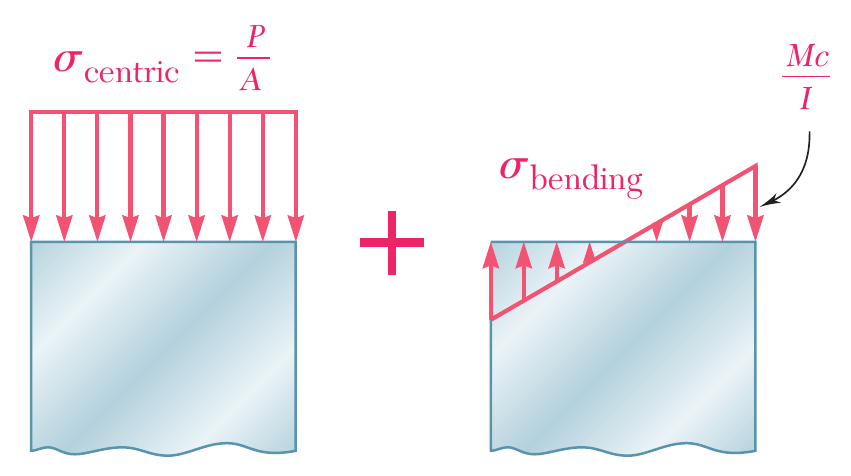
\includegraphics[width=\linewidth,height=2.9cm,keepaspectratio]{Chap_10/fig_10_33.png}
  \end{columns}
\end{frame}

\end{document}
